
\appendix

\chapter{WBS}

\section{Previous WBS}
This is where the Work Breakdown Structures from early development is placed here with the most recent placed earliest, as can be seen in Figures \ref{fig:WBS222}, \ref{fig:WBS13}, \ref{fig:WBS83}, \ref{fig:WBS153}, \ref{fig:WBS223}, \ref{fig:WBS54}, and \ref{fig:WBSfin}.

\begin{figure}[p]
\setlength\fboxsep{0pt}
\setlength\fboxrule{1pt}\noindent\makebox[\textwidth]{%
 \fbox{
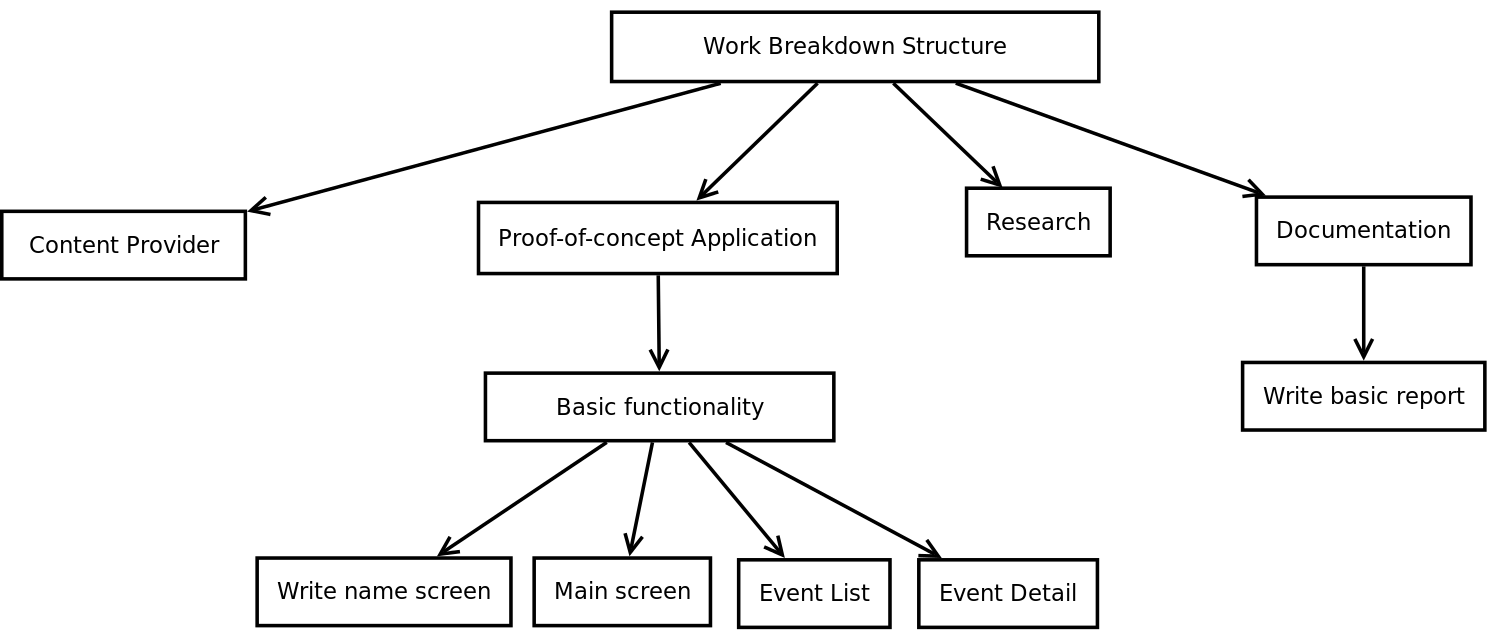
\includegraphics[width=1.45\textwidth , angle=270]{Res/WBSfirst.png}}}
\caption{The WBS as per 22.2.13 }
\label{fig:WBS222}
\end{figure}

\begin{figure}[p]
\setlength\fboxsep{0pt}
\setlength\fboxrule{1pt}\noindent\makebox[\textwidth]{%
 \fbox{
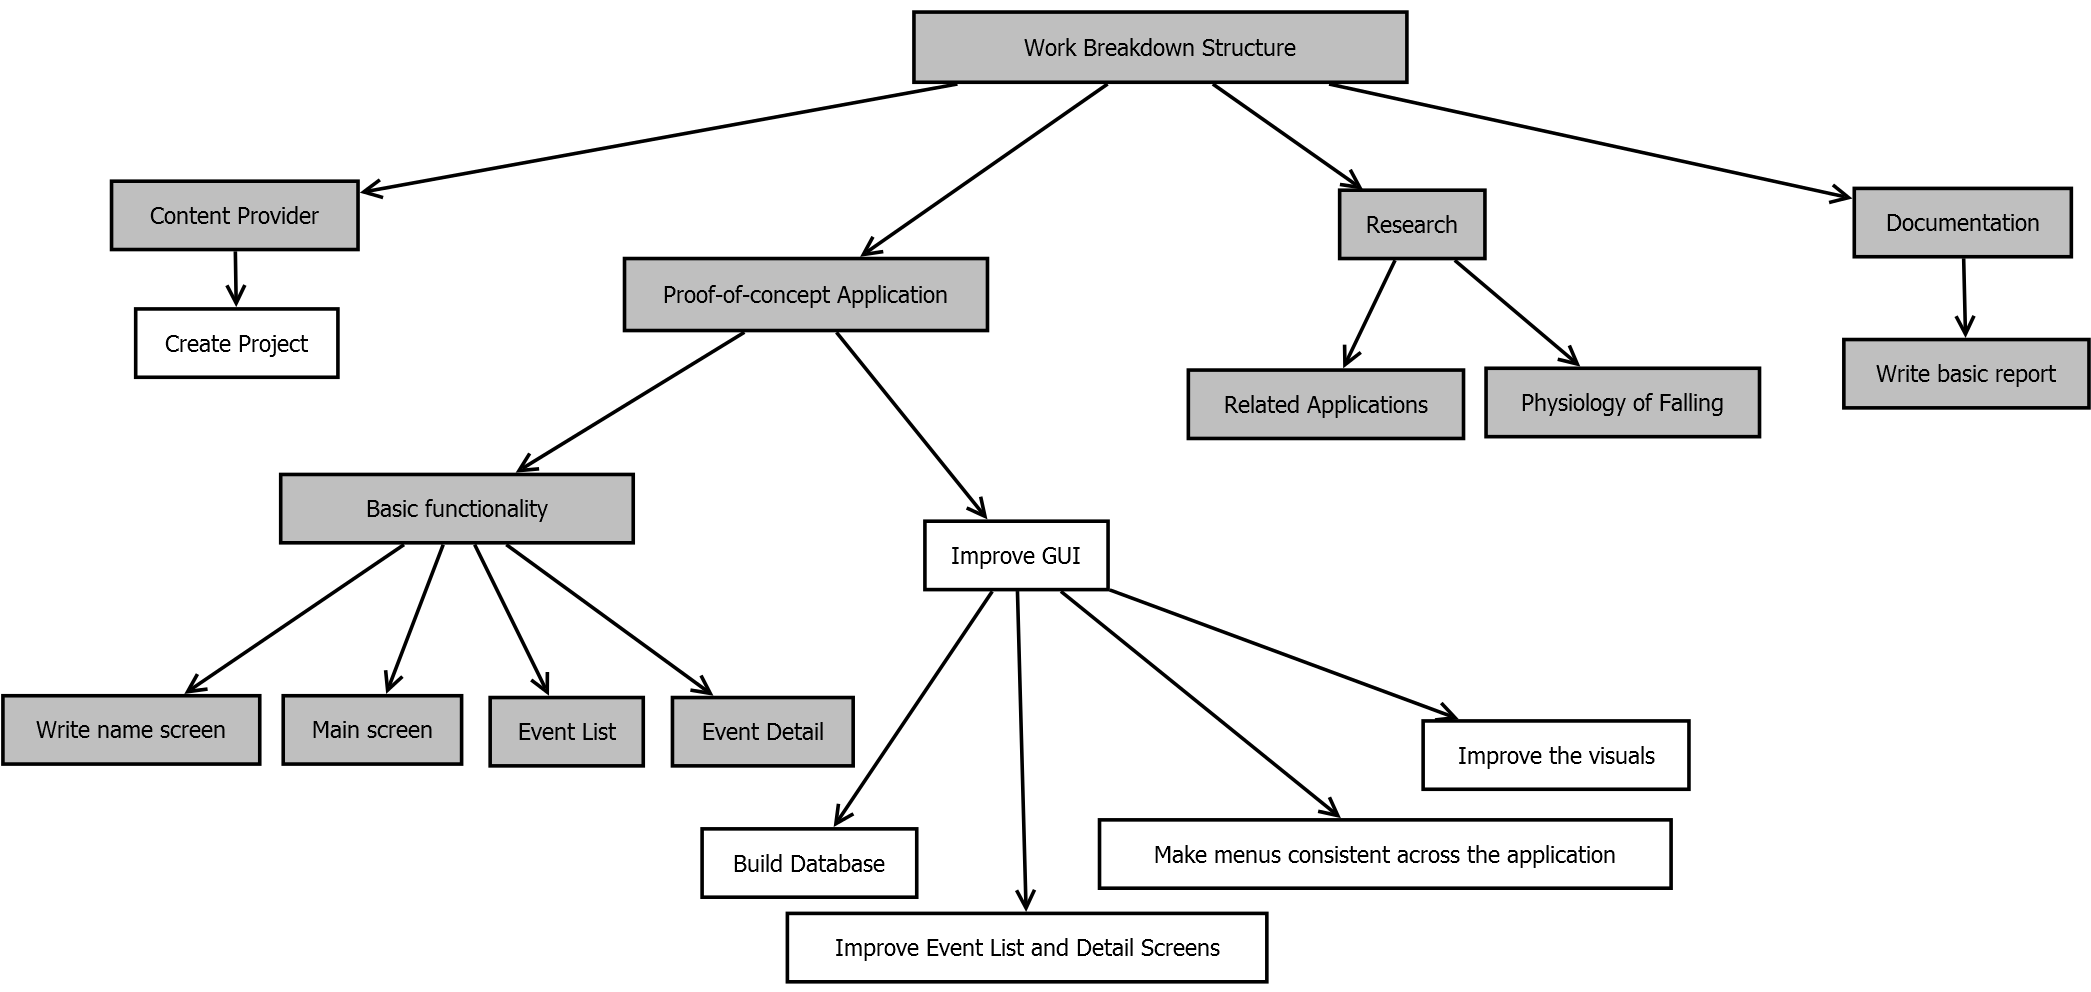
\includegraphics[width=1.45\textwidth , angle=270]{Res/WBS01313.png}}}
\caption{The WBS as per 1.3.13}
\label{fig:WBS13}
\end{figure}


\begin{figure}[p]
\setlength\fboxsep{0pt}
\setlength\fboxrule{1pt}\noindent\makebox[\textwidth]{%
 \fbox{
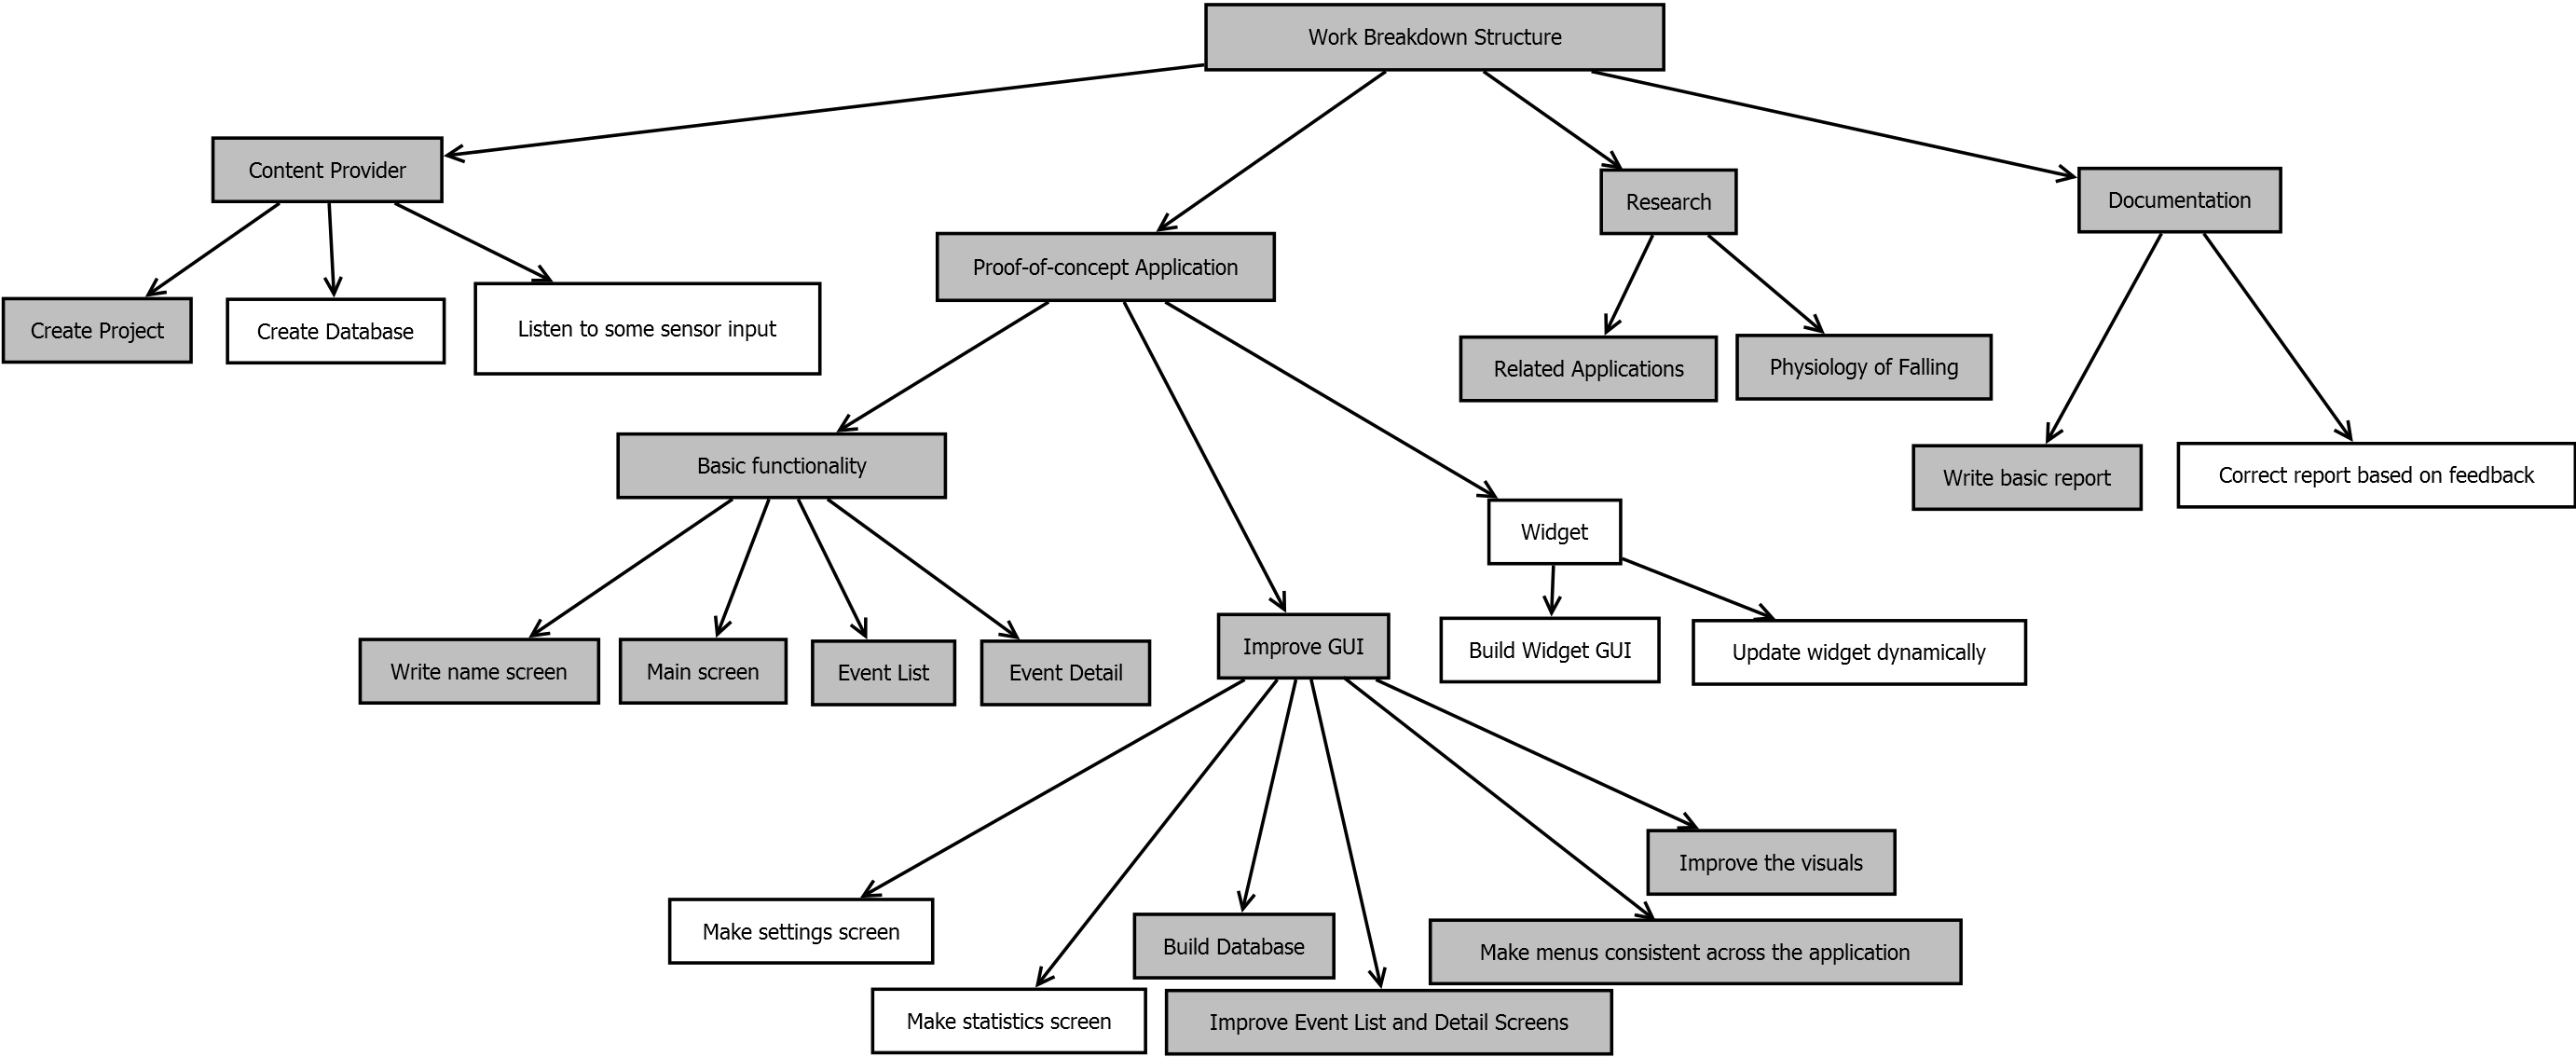
\includegraphics[width=1.45\textwidth , angle=270]{Res/WBS08313.png}}}
\caption{The WBS as per 8.3.13}
\label{fig:WBS83}
\end{figure}

\begin{figure}[p]
\setlength\fboxsep{0pt}
\setlength\fboxrule{1pt}\noindent\makebox[\textwidth]{%
 \fbox{
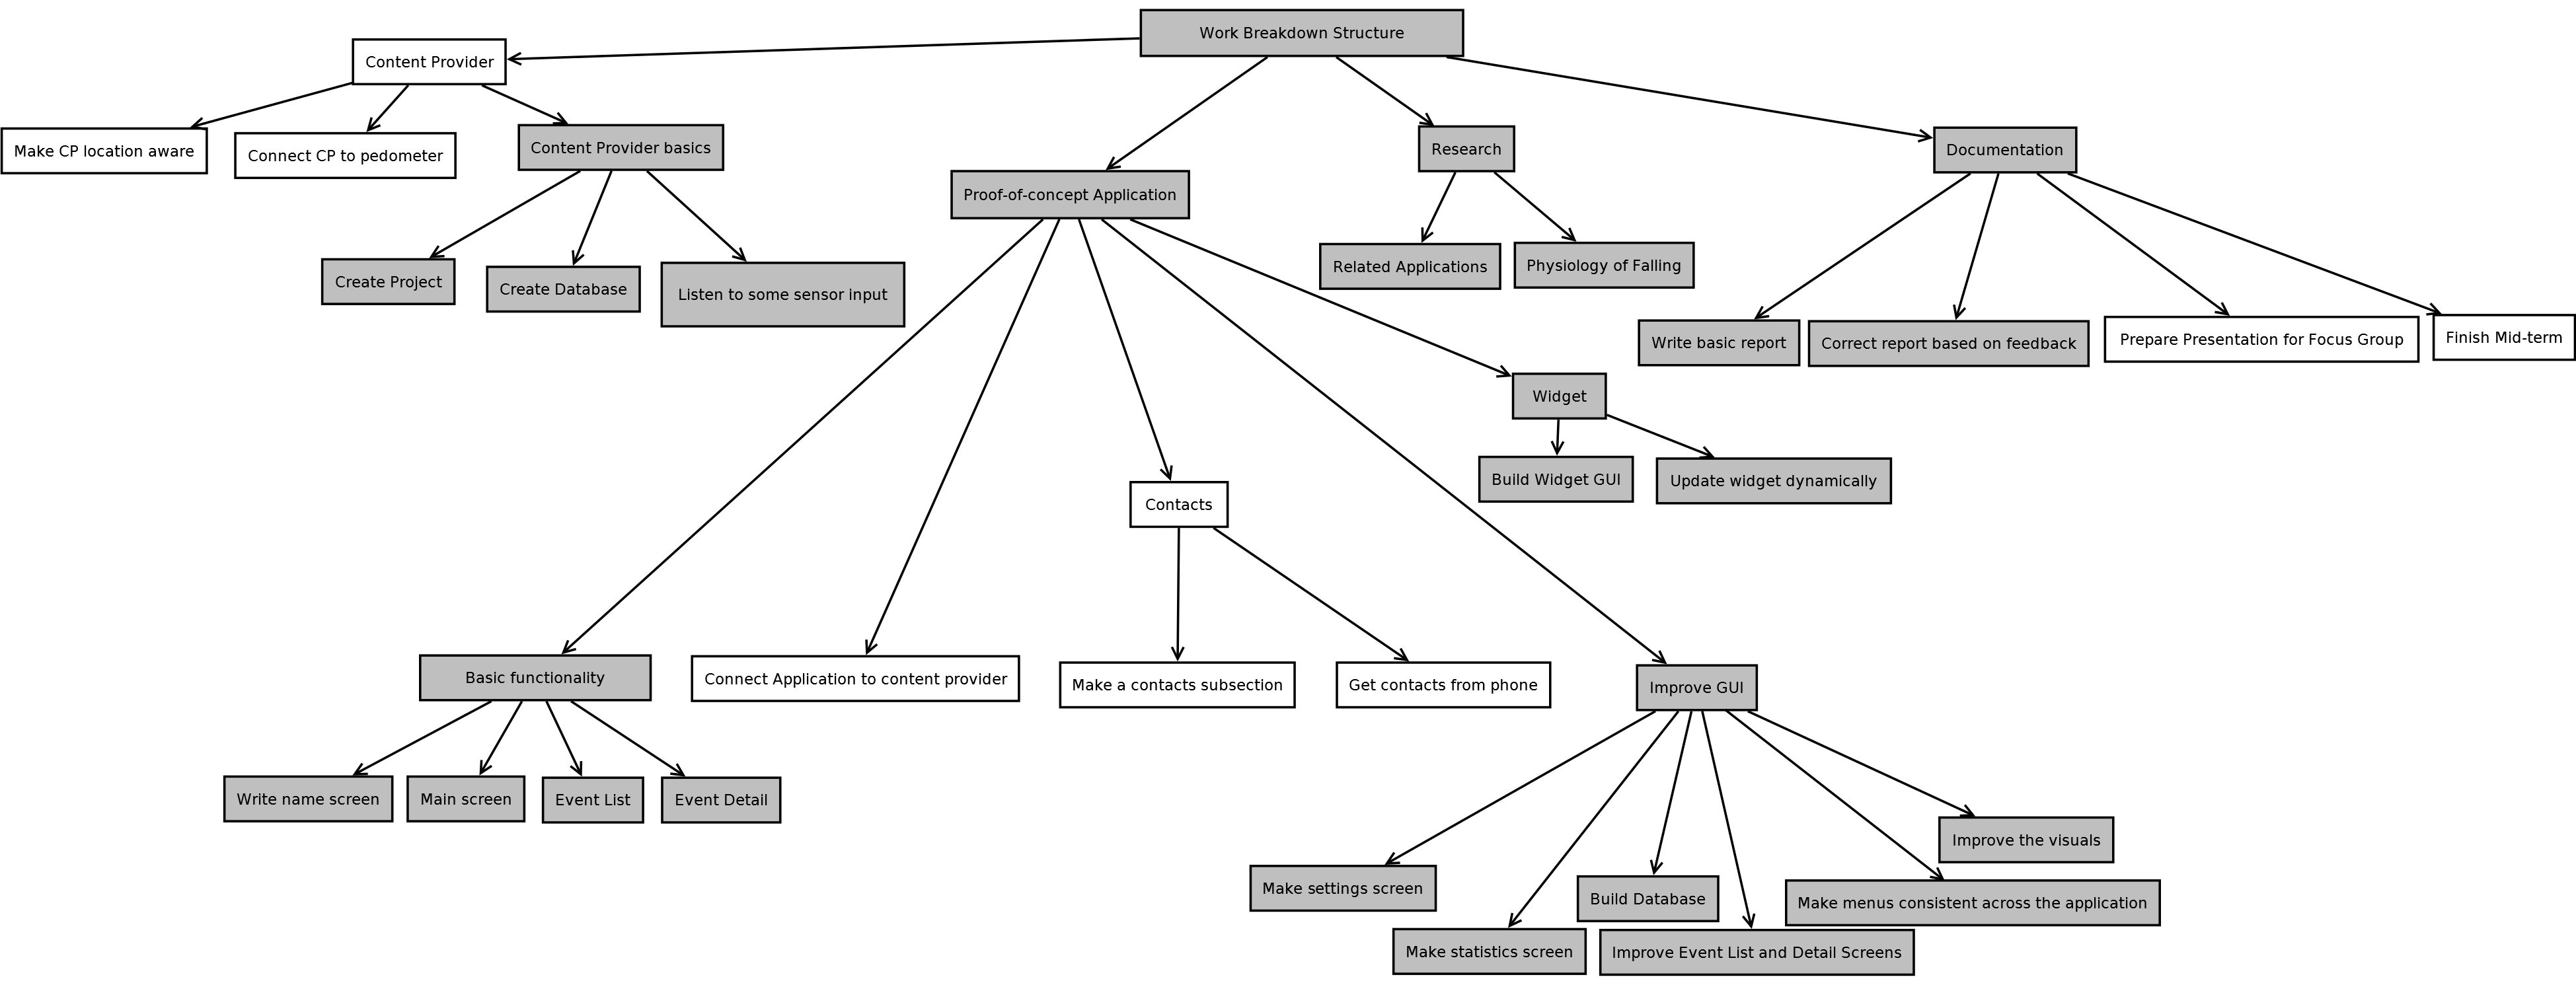
\includegraphics[width=1.45\textwidth , angle=270]{Res/WBS15313.png}}}
\caption{The WBS as per 15.3.13}
\label{fig:WBS153}
\end{figure}

\begin{figure}[p]
\setlength\fboxsep{0pt}
\setlength\fboxrule{1pt}\noindent\makebox[\textwidth]{%
 \fbox{
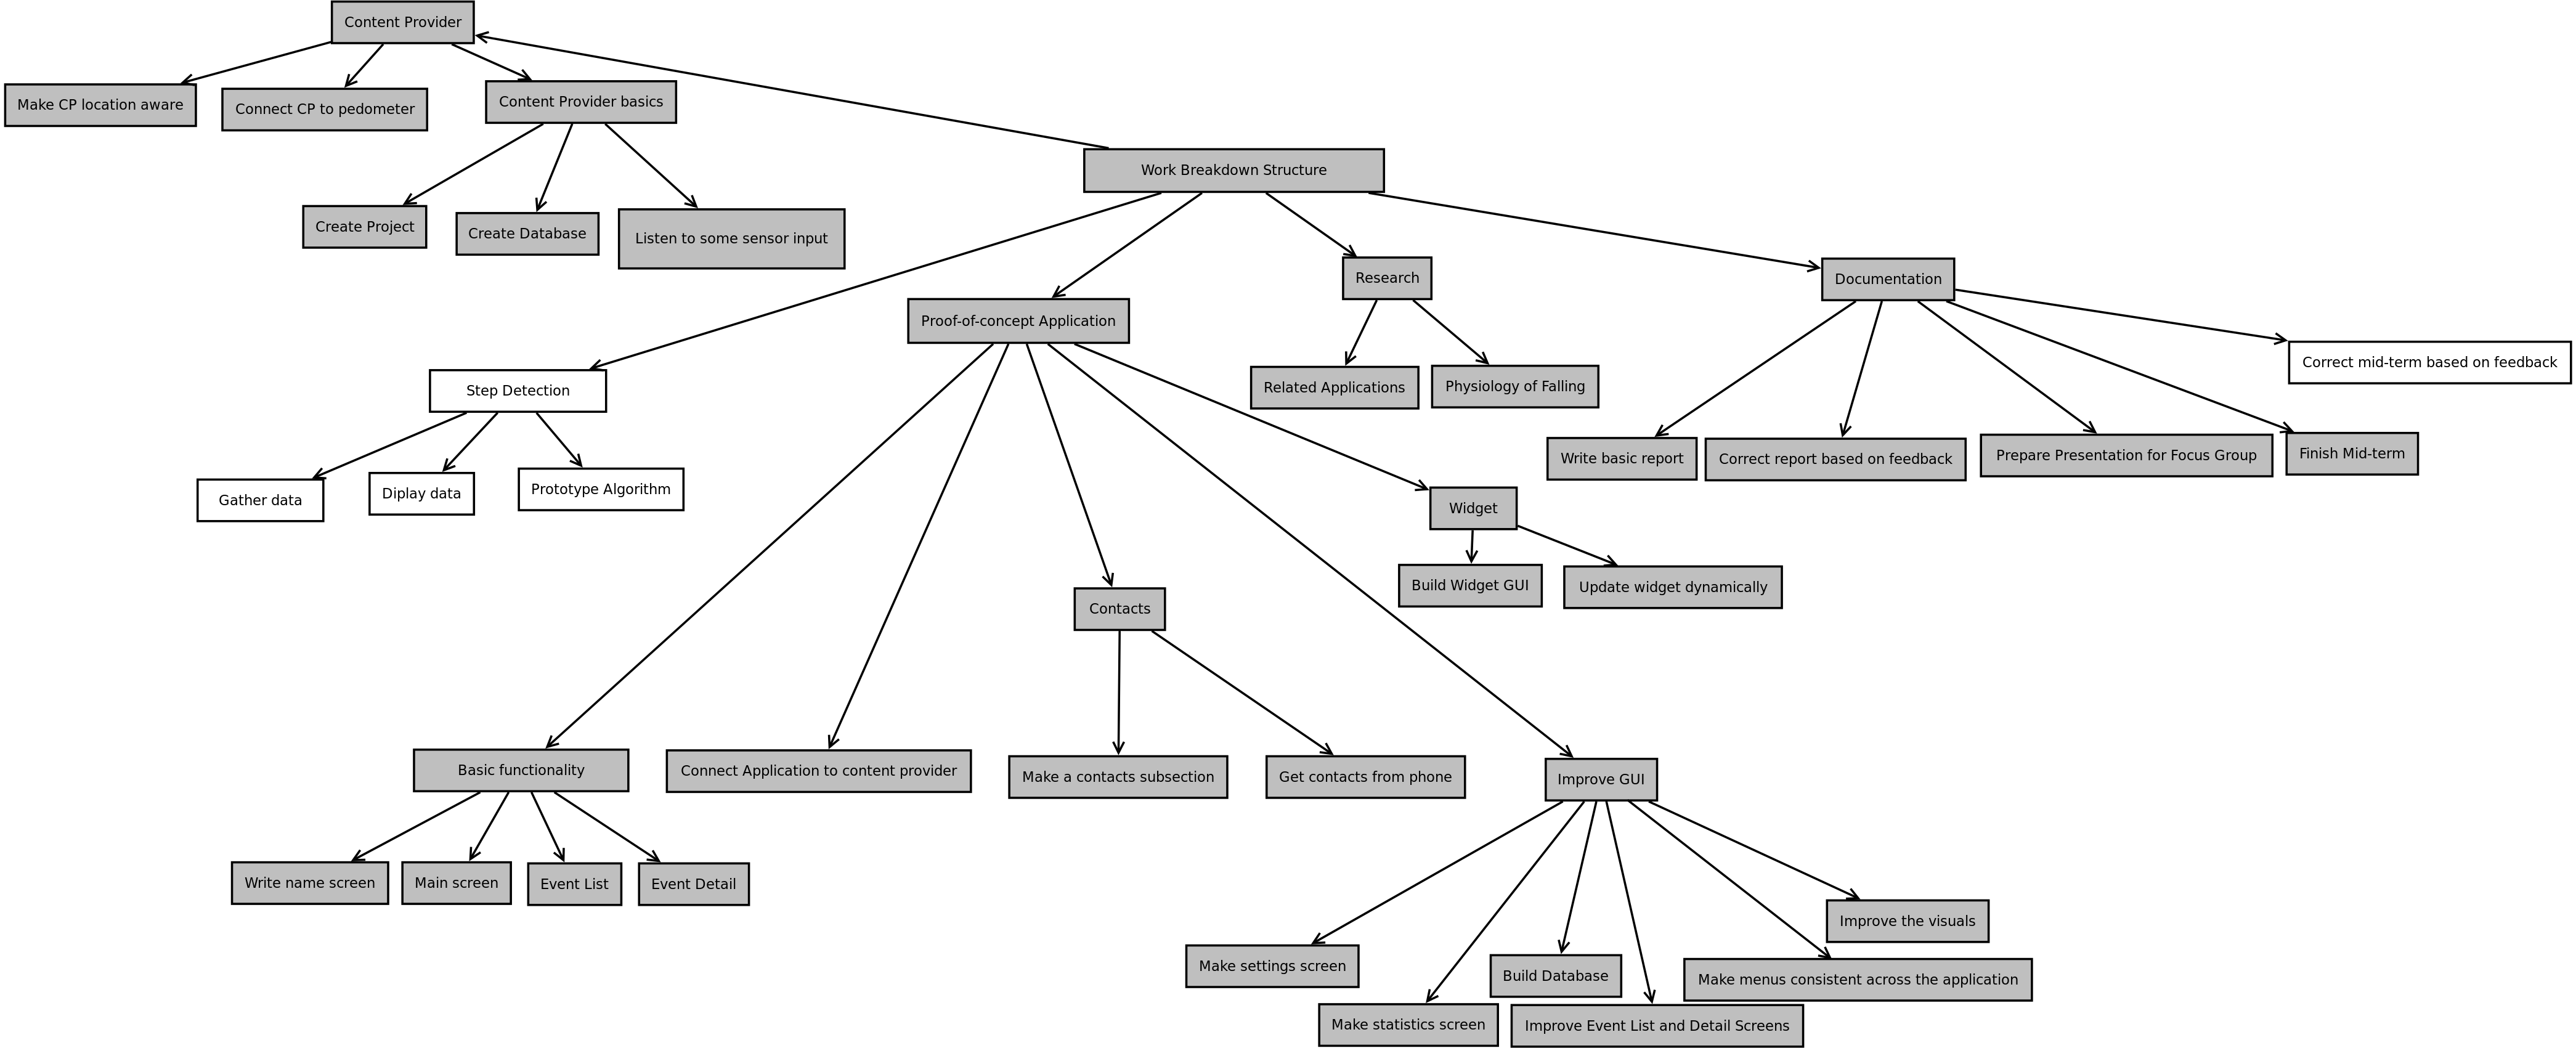
\includegraphics[width=1.45\textwidth , angle=270]{Res/WBS22313.png}}}
\caption{The WBS as per 22.3.13}
\label{fig:WBS223}
\end{figure}

\begin{figure}[p]
\setlength\fboxsep{0pt}
\setlength\fboxrule{1pt}\noindent\makebox[\textwidth]{%
 \fbox{
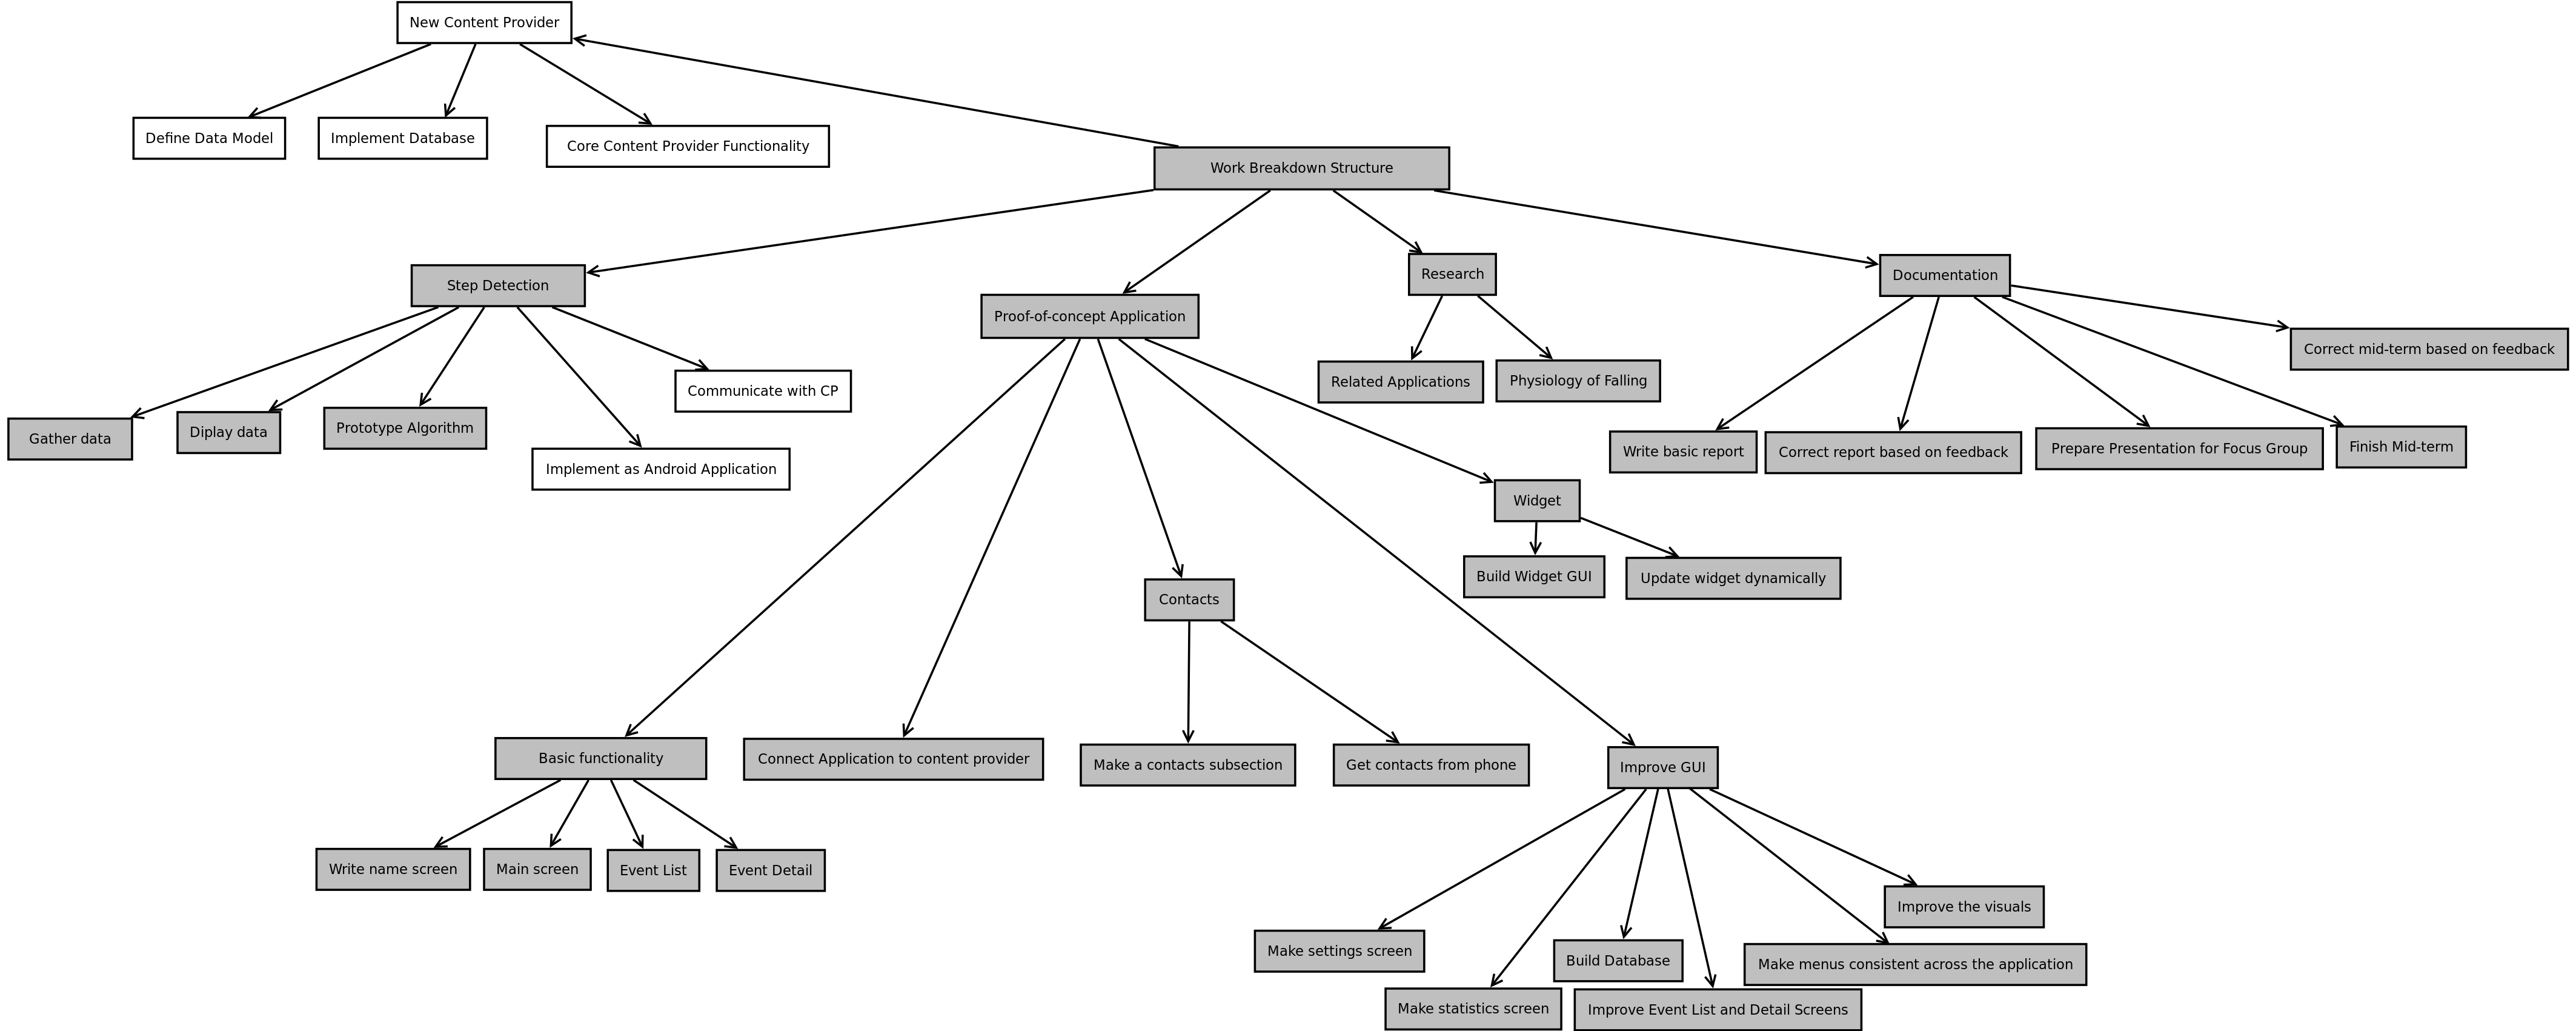
\includegraphics[width=1.45\textwidth , angle=270]{Res/WBS05413.png}}}
\caption{The WBS as per 5.4.13}
\label{fig:WBS54}
\end{figure}

\begin{figure}[p]
\setlength\fboxsep{0pt}
\setlength\fboxrule{1pt}\noindent\makebox[\textwidth]{%
 \fbox{
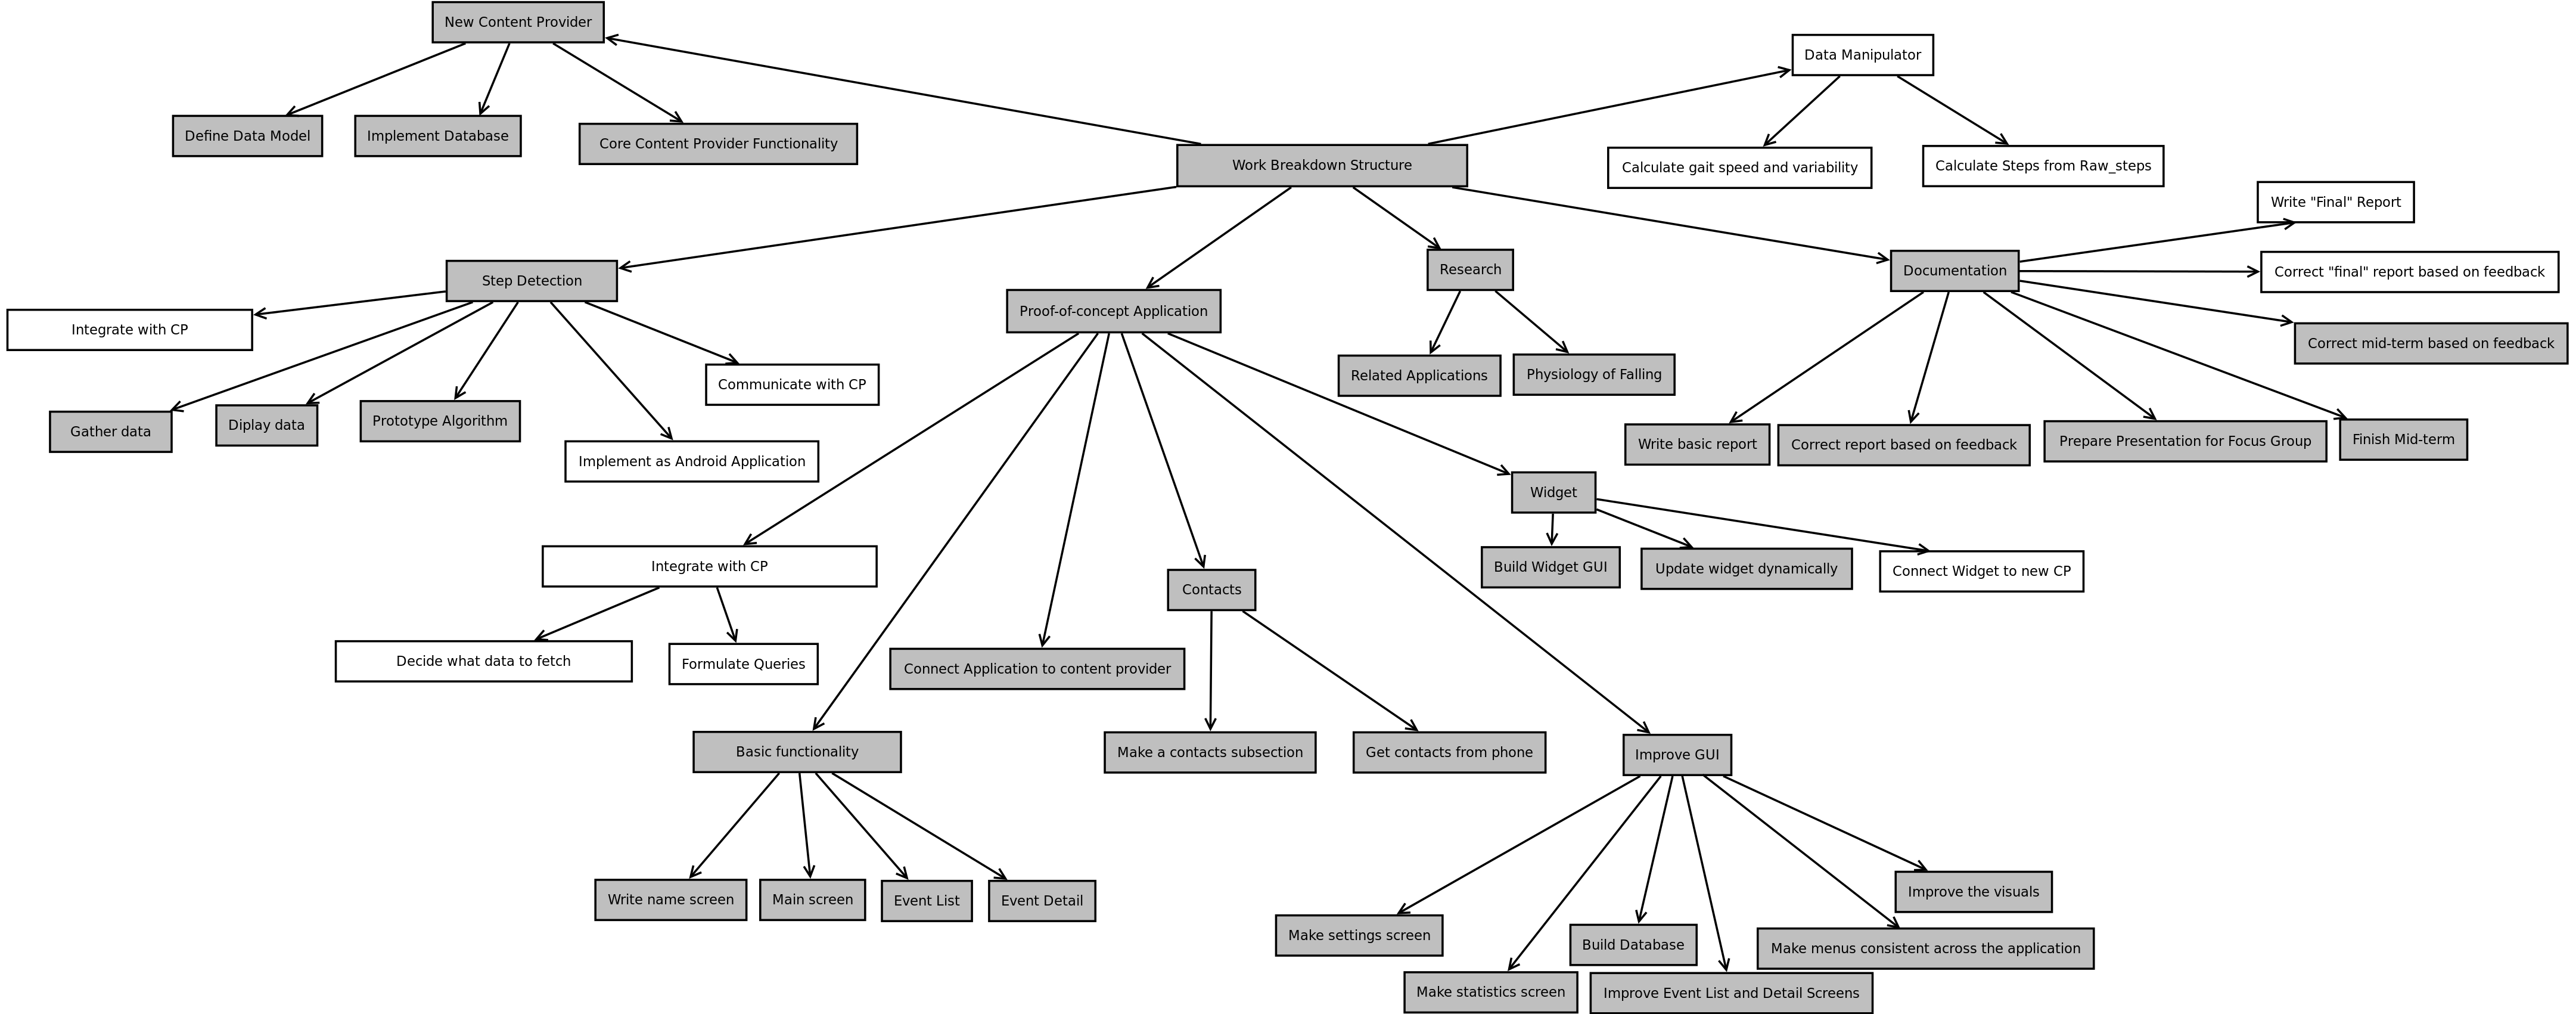
\includegraphics[width=1.45\textwidth , angle=270]{Res/WBSlast.png}}}
\caption{The final WBS}
\label{fig:WBSfin}
\end{figure}

%\section{Reports}

\chapter{Work summary}
\section{Sprint summaries}
\label{tab:sprintList}
The following is a list of the sprints:

\begin{description}
\item[Sprint 1: 01.02.13 - 08.02.13] \hline \hfill \\
User stories and paper prototypes of the GUI were developed.
\item[Sprint 2: 08.02.13 - 15.02.13] \hline \hfill \\
The group focused on learning Android development. New GUI paper prototypes were developed based on customer feedback. A mock-up application demonstrating core parts of the GUI was developed.
\item[Sprint 3: 15.02.13 - 22.02.13] \hline \hfill \\
Continued efforts on learning Android development. The mock-up was developed further. Research was conducted on the application domain, and on related applications. 
\item[Sprint 4: 22.02.13 - 01.03.13] \hline \hfill \\
The prototype application was expanded with a database, GUI visuals were improved, menu usage was made consistent throughout the prototype. The group tried to familiarize themselves with Content Providers in Android.
\item[Sprint 5: 01.03.13 - 08.03.13] \hline \hfill \\
A Content Provider was developed, incorporated the step detection from the Pedometer open-source application. Some secondary screens (settings and statistics) were implemented. Basic widget created.
\item[Sprint 6: 08.03.13 - 15.03.13] \hline \hfill \\
Widget was connected successfully to the main application. Application connected to the Content Provider. Work on report for the mid-term hand-in. Presentation for the focus group prepared. Unsuccessful attempts at making the Pedometer/Content Provider location aware. Implementation of contact management. 
\item[Sprint 7: 15.03.13 - 22.03.13] \hline \hfill \\
Research and development of step detection algorithm: Sensor data collection application developed, python scripts for displaying data and prototyping of algorithm. Work on Javadoc and code refactoring. Correction of report based on mid-term feedback.
\item[Ester holidays: 23.03.13 - 02.04.13] \hline \hfill \\
Little work was done due to the holidays.
\item[Sprint 9: 03.04.13 - 05.04.13] \hline \hfill \\
New system architecture was designed. Step detection algorithm implemented as Android application. The old Content Provider/Pedometer discarded, and new Content Provider implemented. 
\item[Sprint 10: 05.04.13 - 12.04.13] \hline \hfill \\
Efforts were focused on bug-fixing and integration of the three components. 
\item[Sprint 11: 13.04.13 - 19.04.13] \hline \hfill \\
Work on final report and small adjustments the integration of the components. The code underwent refactoring and commenting. 
\end{description}
\section{Meeting summaries}
Regular status reports was a part of necessary documentation. Of particular importance was reports to the supervisor, and reports done to the other group members. This status report was written during sprint 4. The reports were included in chronological order.


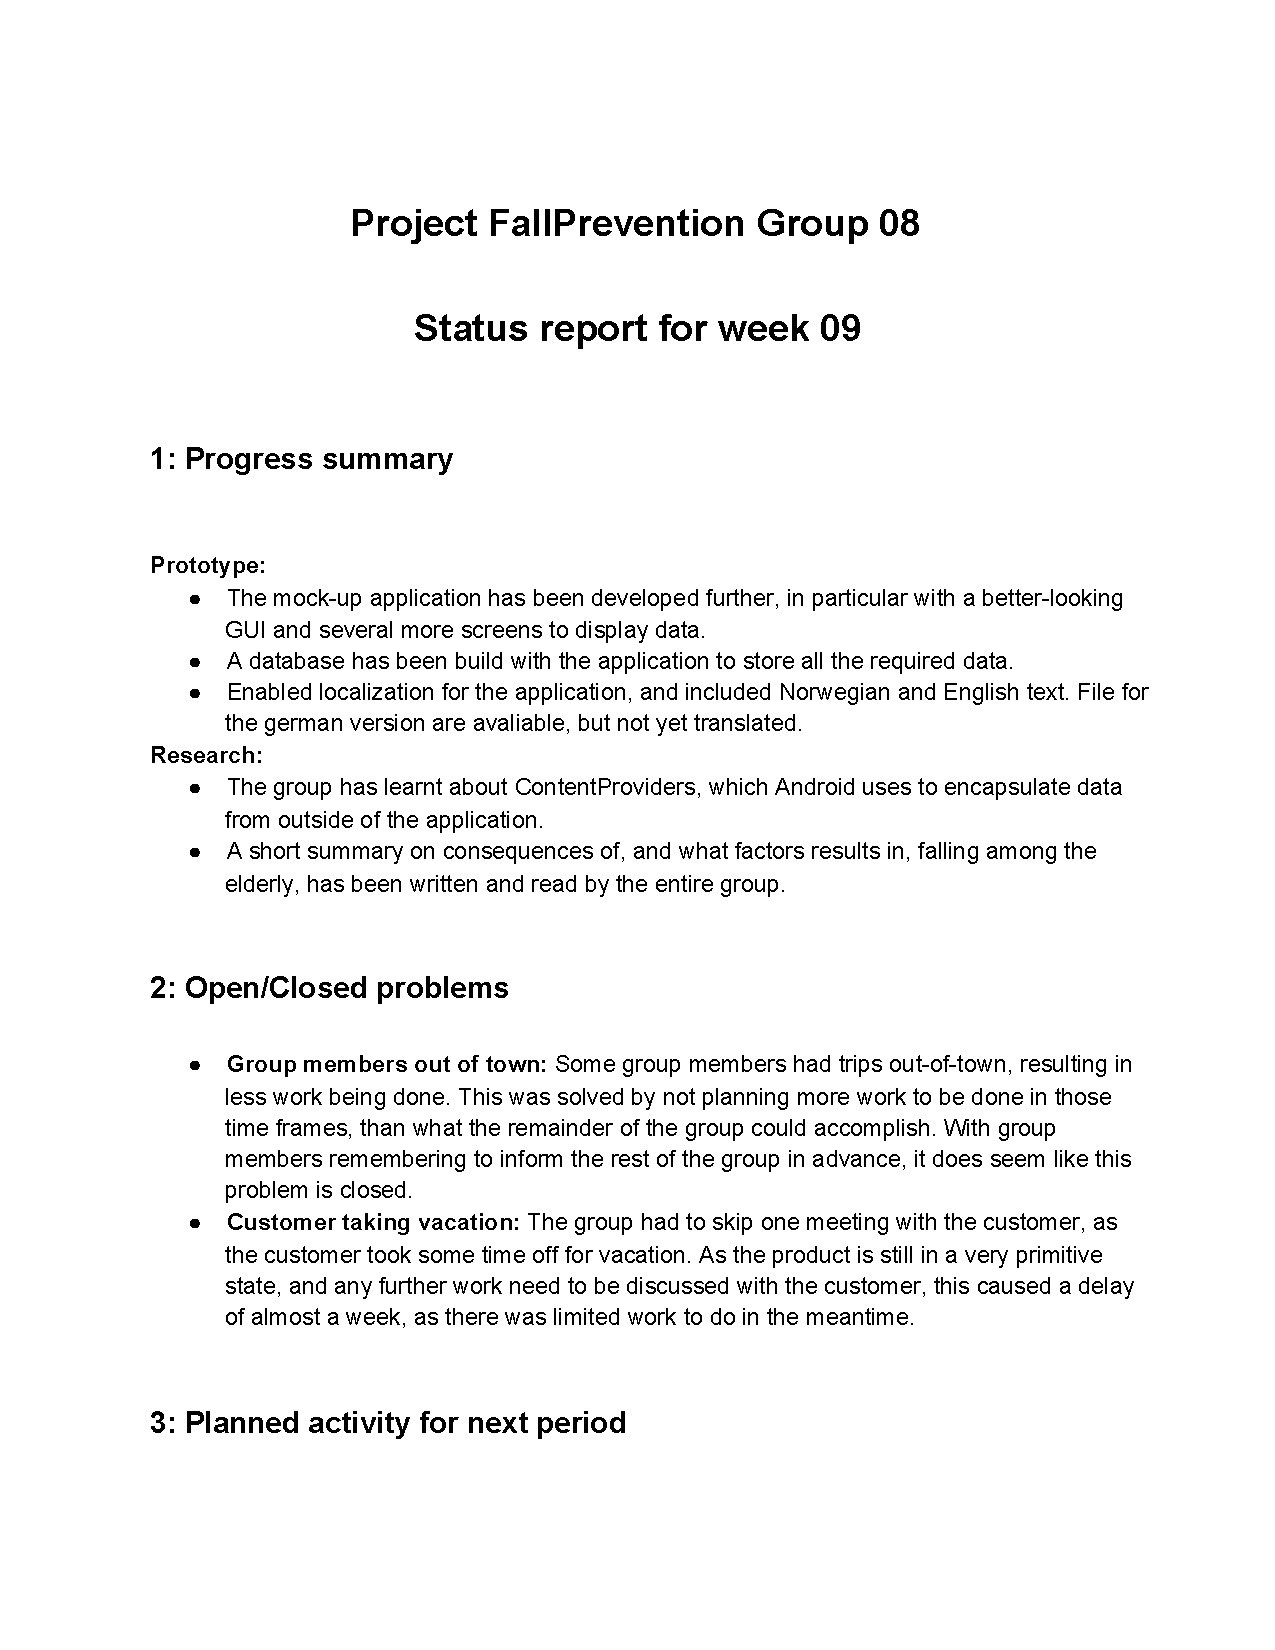
\includepdf[pages={-}]{Res/StatusReportWeek9}

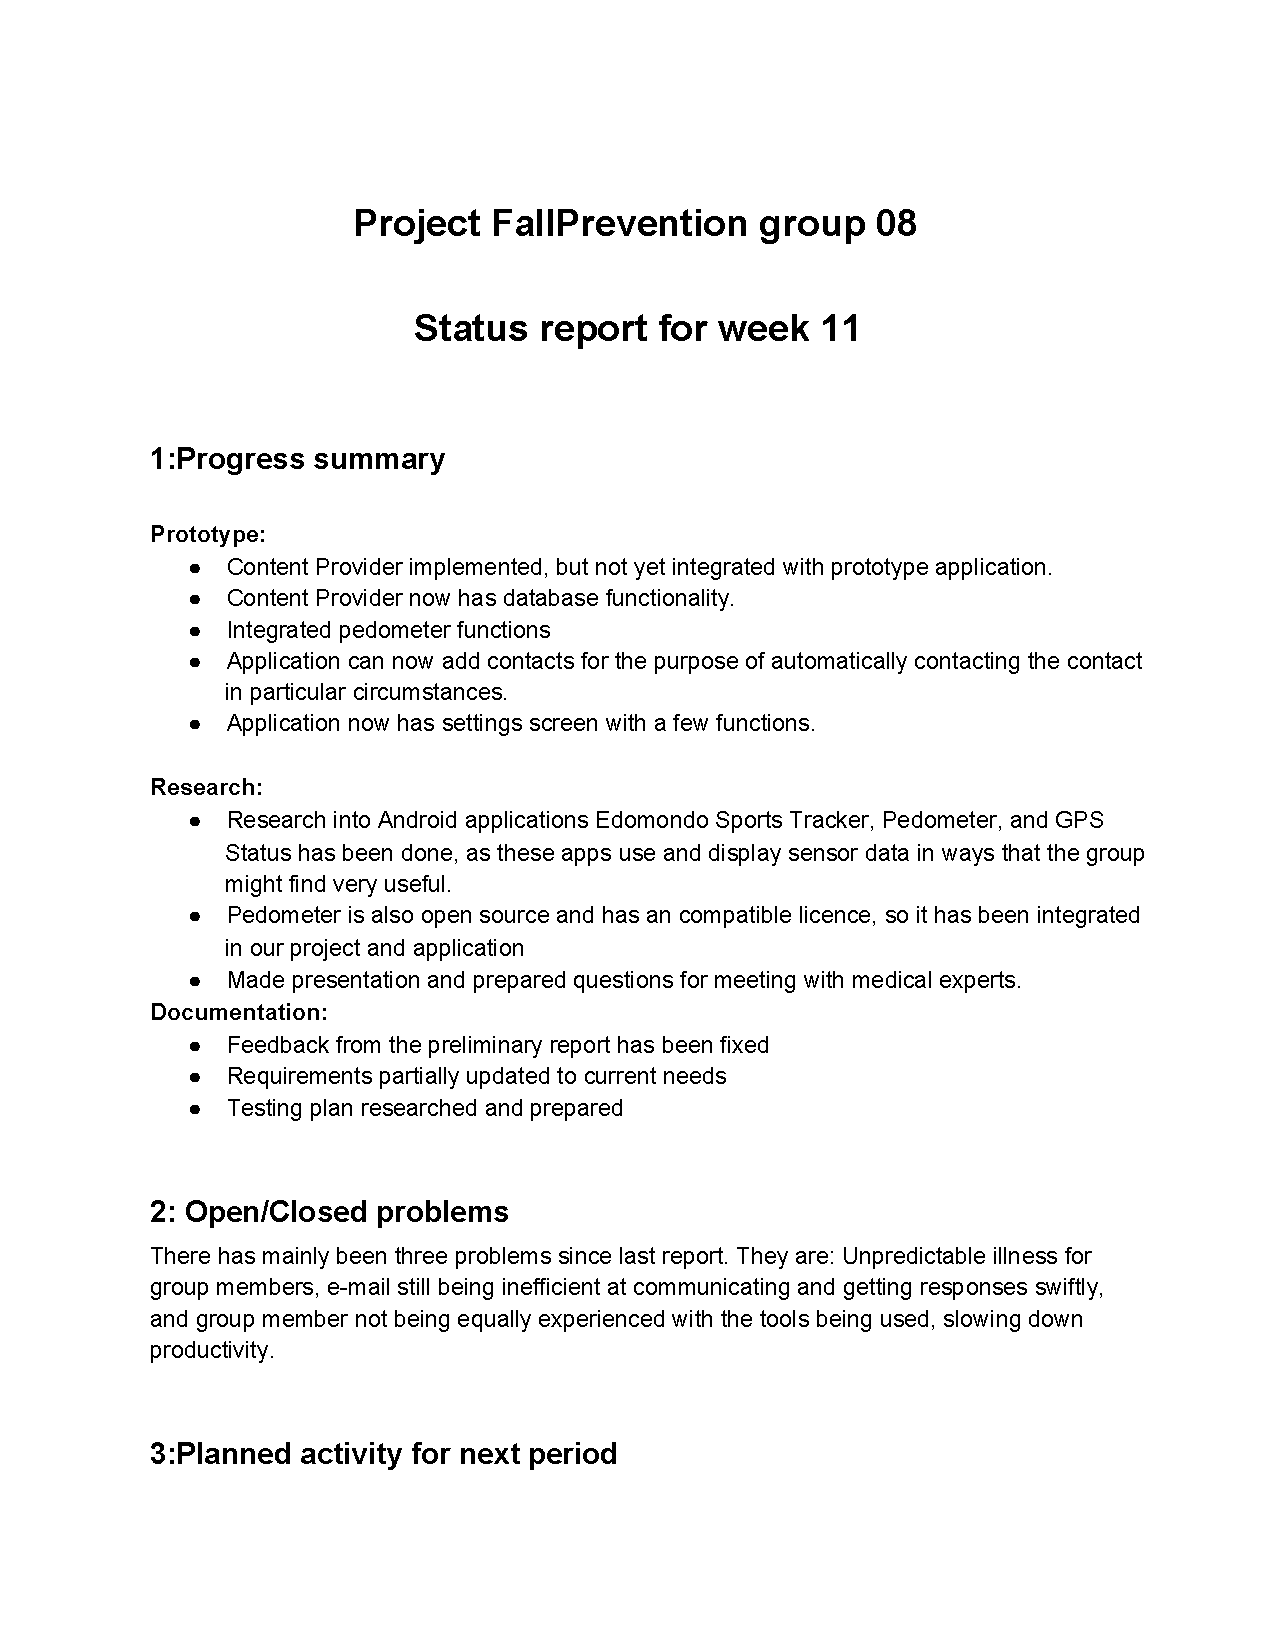
\includepdf[pages={-}]{Res/StatusReportWeek11}

\chapter{Apache License}

\label{appendix:license}
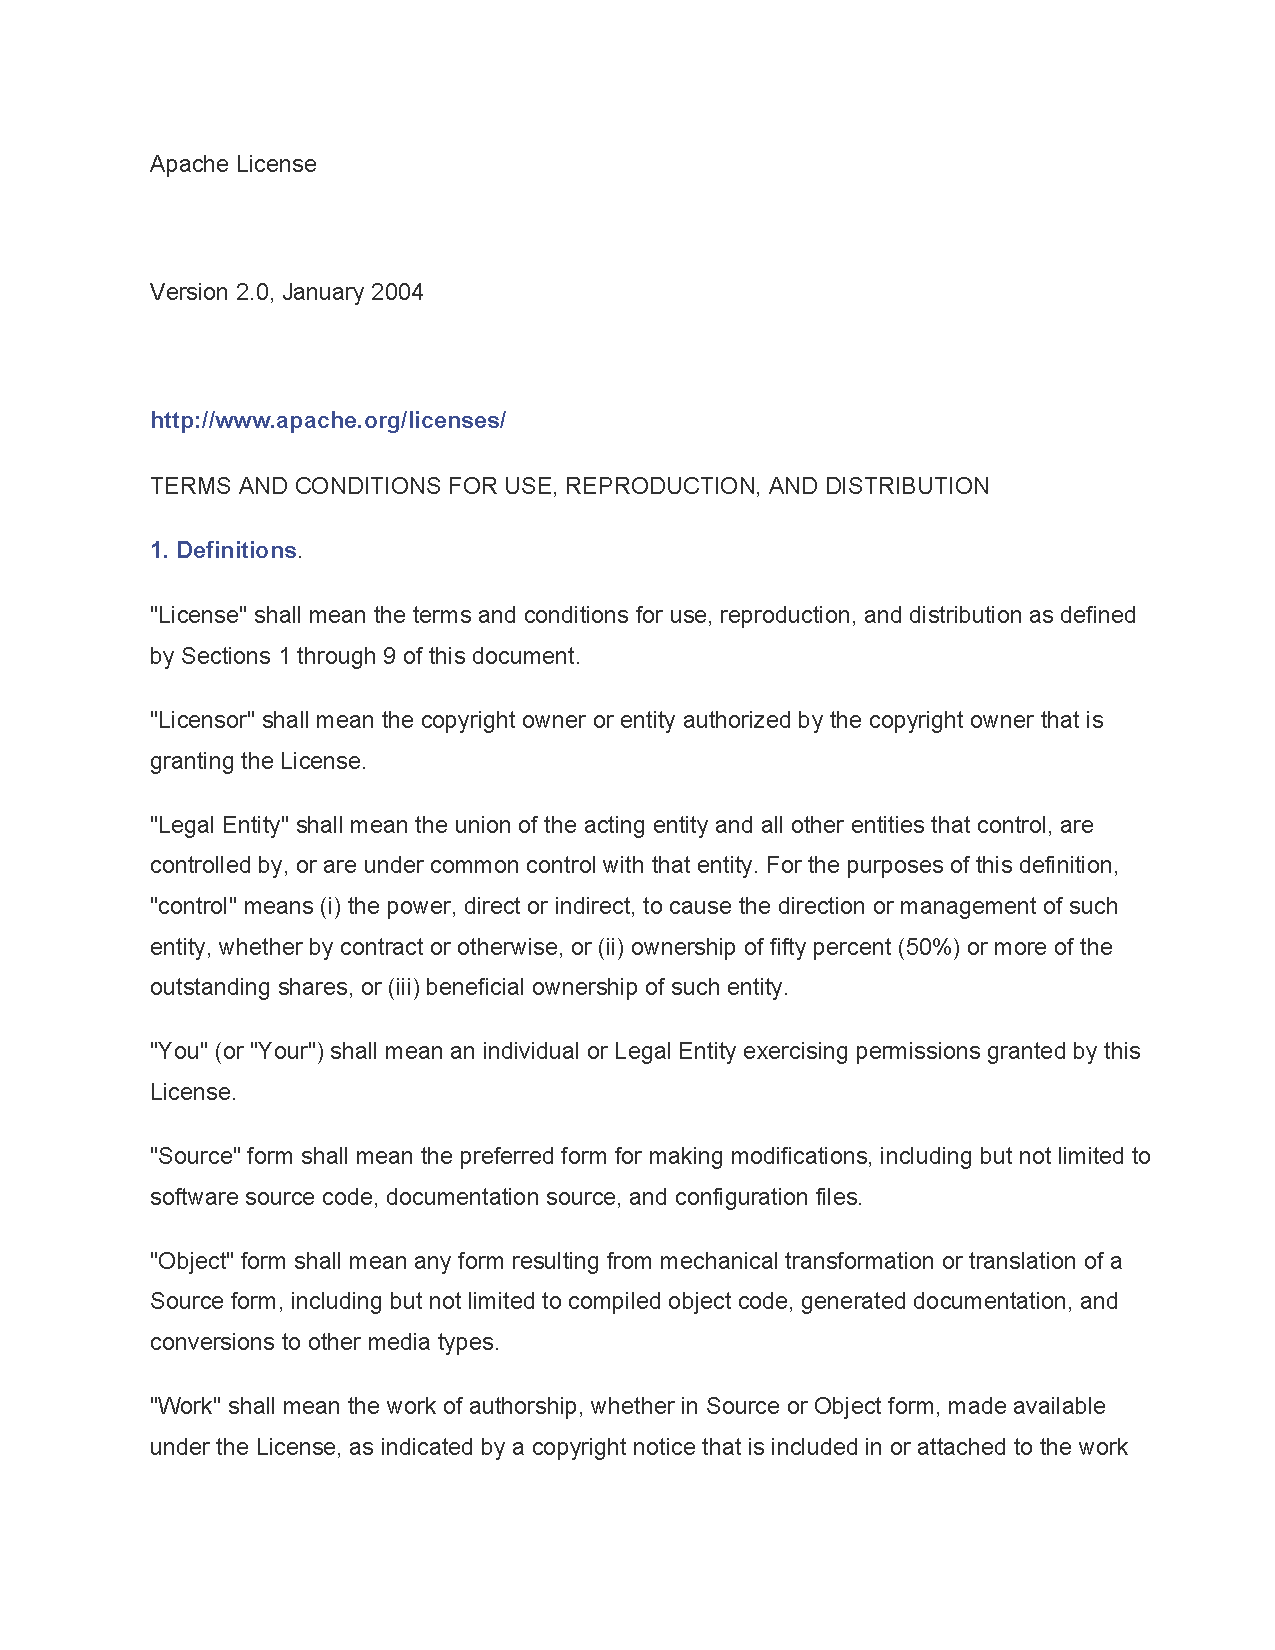
\includepdf[pages={-}]{Res/Apache2license}


\chapter{Test results}
Here is a copy of feedback the group received from the customer when the application was deployed for testing. 
\label{appendix:testResults}
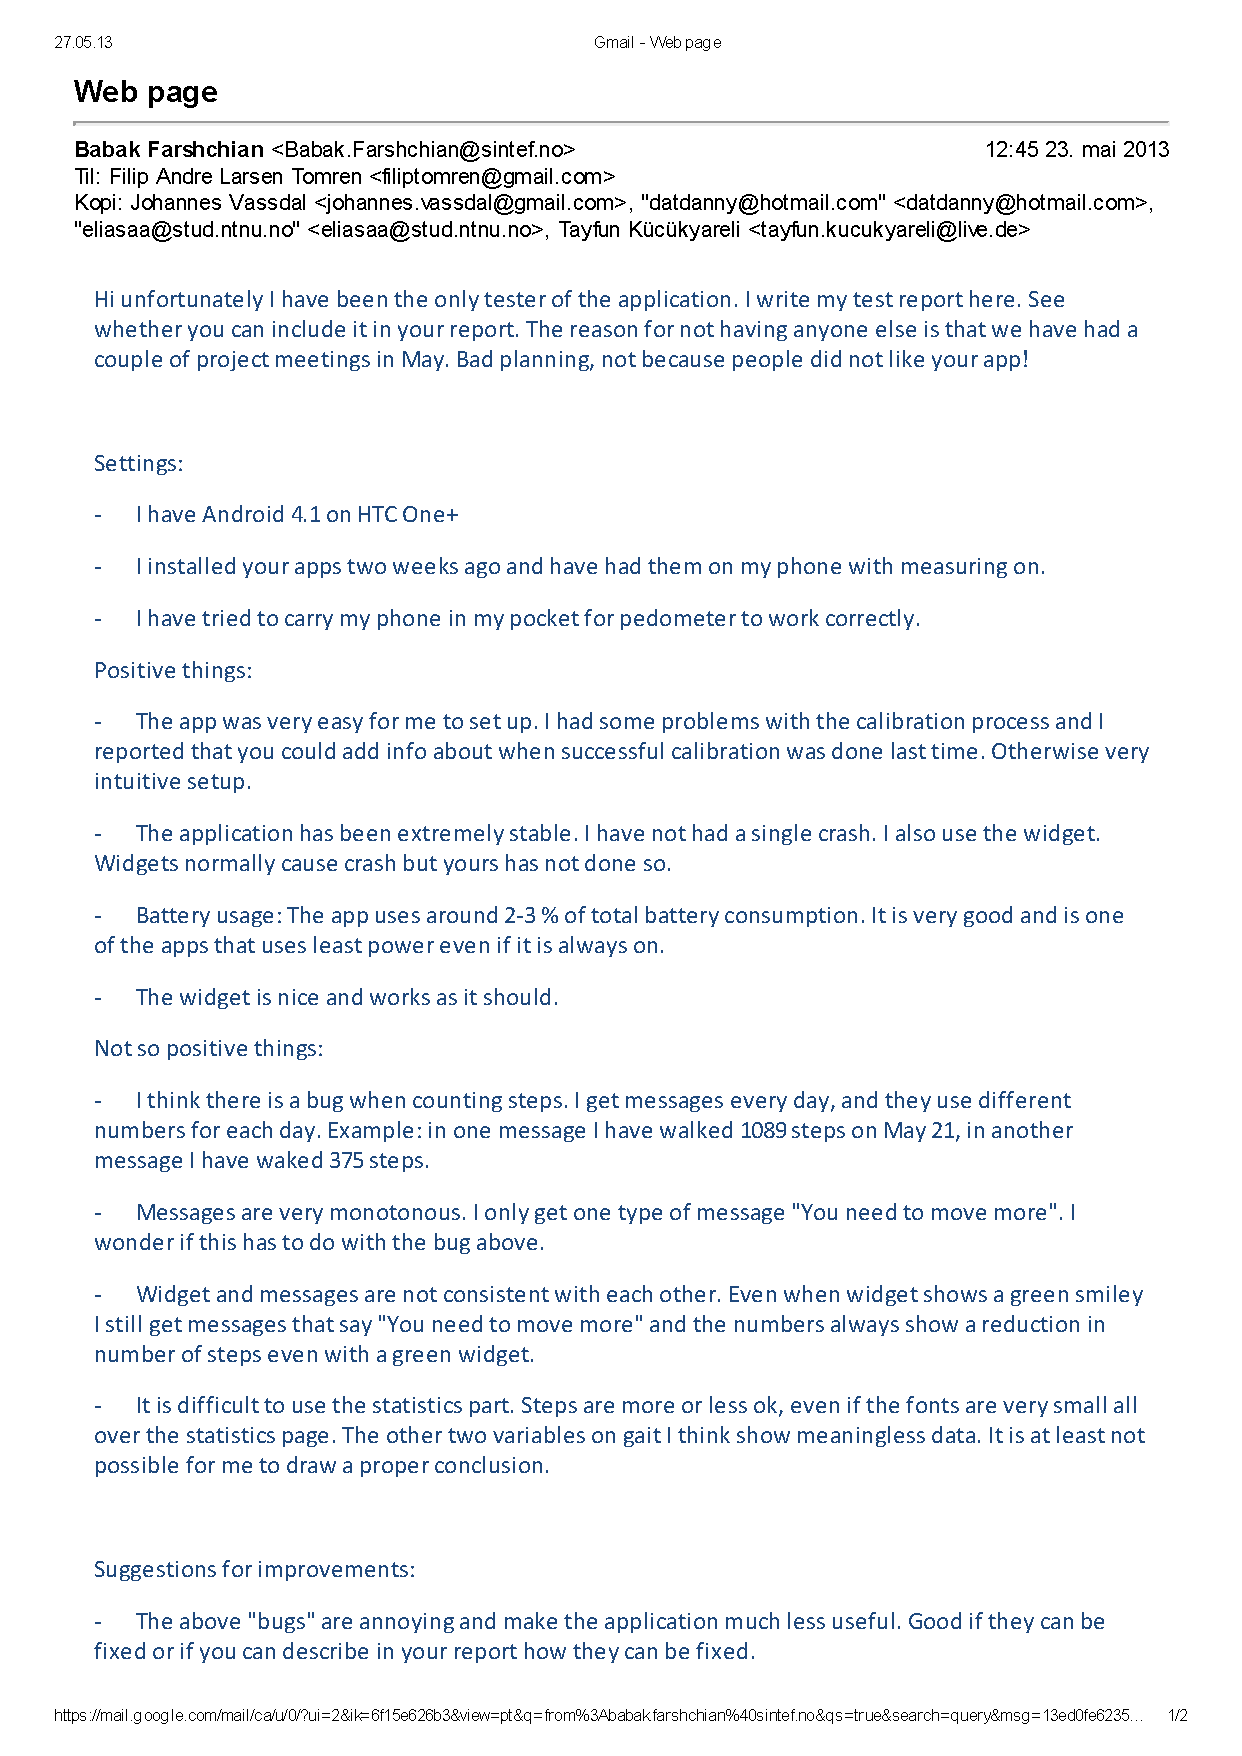
\includepdf[pages={-}]{Res/TestingSummaryBabak}

\chapter{Time-sheet}
Here is the time-sheet used to log time spent working on the project.
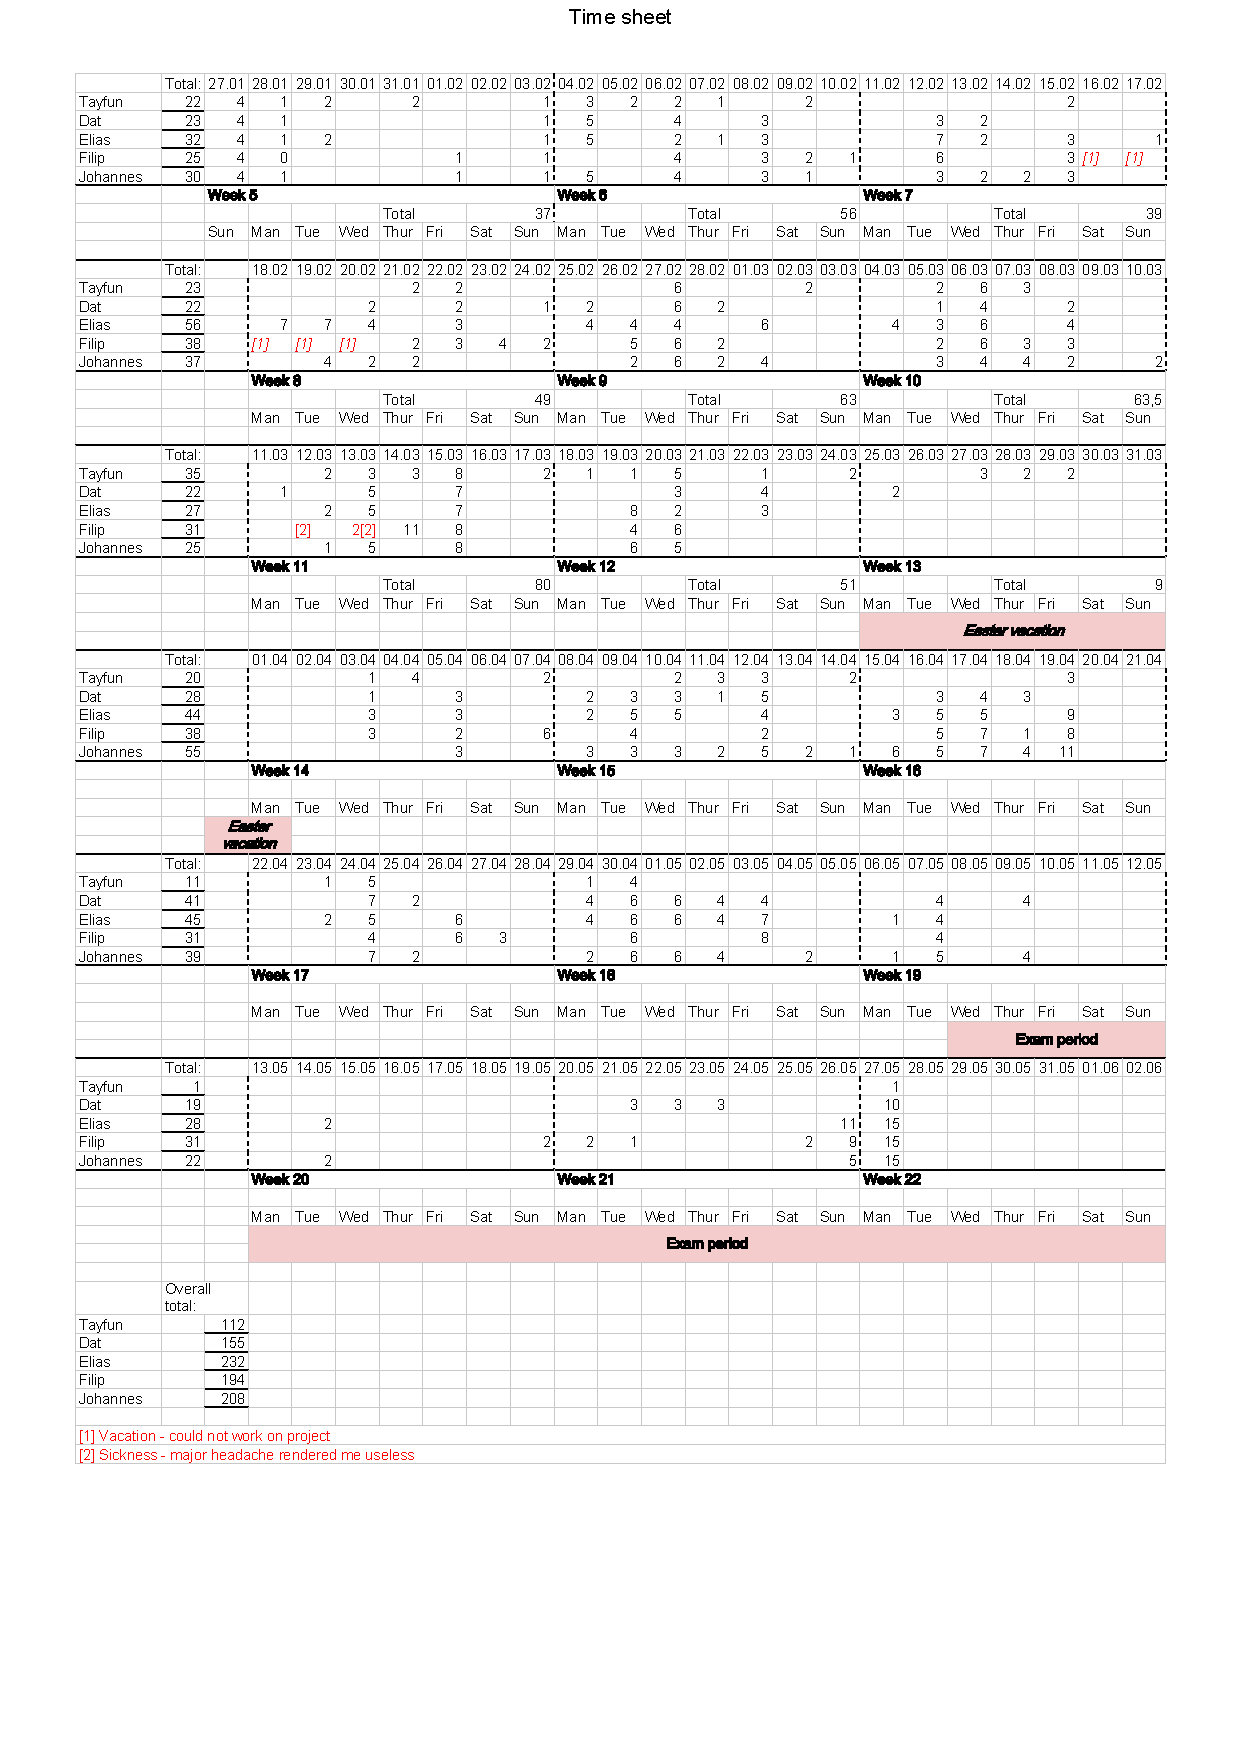
\includepdf[pages={1}]{Res/TimeSheet}





